\documentclass[a4paper]{ltjsarticle}

\usepackage[dvipdfmx]{graphicx}
\usepackage[dvipdfmx,hidelinks,pdfusetitle]{hyperref}
\hypersetup{
    colorlinks=false,
    bookmarksnumbered=true,
    pdfborder={0 0 0},
    bookmarkstype=toc
}
\usepackage[nobreak]{cite}
\usepackage{pxjahyper}
\usepackage{amsmath}
\usepackage{tikz}

\usetikzlibrary{datavisualization}
\usetikzlibrary{positioning}
\usetikzlibrary{shapes.geometric, shapes.misc}
\usetikzlibrary{patterns}
\usetikzlibrary{calc}

\begin{document}

\begin{itembox}[l]{京都大学 2017年 文系 第1問}

    $w$ を0でない複素数,$x$,$y$ を $w+\frac{1}{w}=x+yi$ を満たす実数とする。

    \begin{enumerate}[label=(\arabic*)]
        \item 実数 $R$ は $R>1$ を満たす定数とする。$w$ が絶対値 $R$ の複素数全体をうごくとき,$xy$ 平面上の点 $(x,y)$ の軌跡を求めよ。
        \item 実数 $\alpha$ は $0<\alpha<\pi/2$ を満たす定数とする。$w$ が偏角 $\alpha$ の複素数全体をうごくとき,$xy$ 平面上の点 $(x,y)$ の軌跡を求めよ。
    \end{enumerate}
\end{itembox}

\begin{enumerate}[label=(\arabic*)]
    \item
          \begin{equation}
              w+\frac{1}{w}=x+yi\label{eq:1}
          \end{equation}

          $w=R(\cos\theta+i\sin\theta)\ (0\leq \theta<2\pi)$ とおけて,\eqref{eq:1}式に代入すると,

          \begin{equation*}
              x+yi=R(\cos\theta+i\sin\theta)+\frac{1}{R(\cos\theta+i\sin\theta)}=R(\cos\theta+i\sin\theta)+\frac{1}{R}(\cos\theta-i\sin\theta)
          \end{equation*}

          $x, y, R, \theta$ は実数より,

          \begin{equation}
              x=\qty(R+\frac{1}{R})\cos\theta,\quad y=\qty(R-\frac{1}{R})\sin\theta\label{eq:2}
          \end{equation}

          $R>1$ より,

          \begin{equation}
              R+\frac{1}{R}>R-\frac{1}{R}>0\label{eq:3}
          \end{equation}

          \eqref{eq:2}式,\eqref{eq:3}式と $0\leq \theta<2\pi$ より,点 $(x,y)$ の軌跡は

          \begin{equation*}
              \frac{x^2}{\qty(R+\frac{1}{R})^2}+\frac{y^2}{\qty(R-\frac{1}{R})^2}=1
          \end{equation*}

    \item $w=r(\cos\alpha+i\sin\alpha)\ (r>0)$ とおけて,\eqref{eq:2}式と同様にして,

          \begin{align}
              x & =\qty(r+\frac{1}{r})\cos\alpha\label{eq:4} \\
              y & =\qty(r-\frac{1}{r})\sin\alpha\label{eq:5}
          \end{align}

          \eqref{eq:4}式,\eqref{eq:5}式より,$r$ を消去すると,

          \begin{equation}
              \qty(\frac{x}{\cos\alpha})^2-\qty(\frac{y}{\sin\alpha})^2=4\quad\Longleftrightarrow\quad \frac{x^2}{(2\cos\alpha)^2}-\frac{y^2}{(2\sin\alpha)^2}=1\label{eq:6}
          \end{equation}

          次に,$rt$ 平面上で,

          \begin{equation*}
              t=r+\frac{1}{r},\quad t=r-\frac{1}{r}\quad (r>0)
          \end{equation*}

          のグラフは下図である。

          \begin{figure}[!ht]
              \centering
              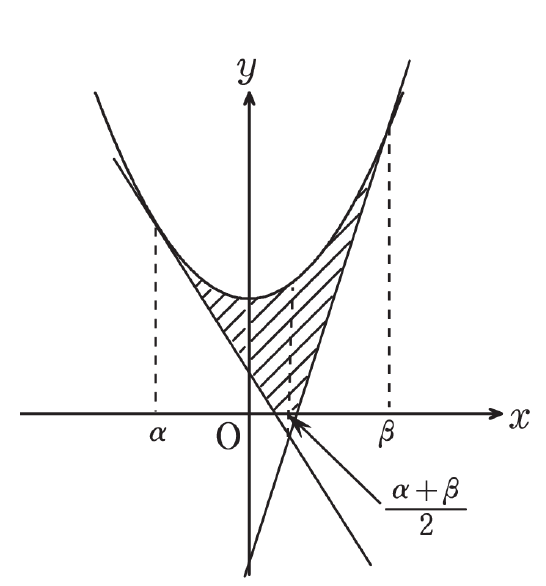
\includegraphics[width=100mm]{f1.png}
          \end{figure}

          よって,\eqref{eq:4}式,\eqref{eq:5}式より,$x$,$y$の取り得る値の範囲は,$0<\alpha<\pi/2$ より,

          \begin{equation}
              x\geq 2\cos\alpha,\quad y\text{は全実数}\label{eq:7}
          \end{equation}

          \eqref{eq:6}式,\eqref{eq:7}式より,点 $(x,y)$ の軌跡は,

          \begin{equation*}
              \frac{x^2}{(2\cos\alpha)^2}-\frac{y^2}{(2\sin\alpha)^2}=1\text{の}x>0\text{の部分}
          \end{equation*}
\end{enumerate}

\end{document}
